\newpage
\chapter*{Taylor'd UI}
\addcontentsline{toc}{chapter}{1. Taylor'd UI}
% Chapter for each research question
% how we validated it and proved it worked

Taylor'd UI is a full \gls{UI} framework that is aimed towards an entry level user. The framework is non-opinionated, light weight, easy to understand, theme-able, and most importantly easy to learn. 

The vocabulary used in Taylor'd UI has been designed to be user friendly so that when a user reads the syntax, they should have an idea of what the end result will look like without writing any code. The vocabulary follows english terminology, for example a pill shaped buttons syntax is: 

\begin{lstlisting}[language=HTML]
<button class="pill-shaped-button">Button</button>
\end{lstlisting}

Taylor'd UI has minimal styling, styling has only been added where needed. That styling is kept to basic colours. This was to ensure the framework does not carry the design opinions of the developer. Being non-opinionated, Taylor'd UI is intensionally bare so that the end user is encouraged to not rely upon the built-in styling, but instead to use it as a starting point to build upon it. 

One of the aims is to make the library as small as possible to ensure it loads quickly on mobile devices and in situations where fast network connectivity is not available. This also ensures that the data used on mobile devices is not unnecessarily burdened.

To stop code from being repeated unnecessarily, code sections have been broken into partials to allow for the ability for the content to be broken up into manageable pieces, removing receptive code such as headers, and footers.

Taylor'd UI is made up of the following features; typography, buttons, alerts, tables, panels, jumbotron, button groups, forms, and a responsive 12 grid system.

\newpage
\subsection*{Typography}
\addcontentsline{toc}{subsection}{1.1 Typography}
The typography used in Taylor'd UI is Open Sans. The default font size throughout the document is 16. There are text modifiers such as extra-small-p, and extra-large-p that decrease or increase the font size as seen on Figure.~\ref{fig:fontSize} on  page~\pageref{fig:fontSize}. 

\begin{figure}[h]
\centering
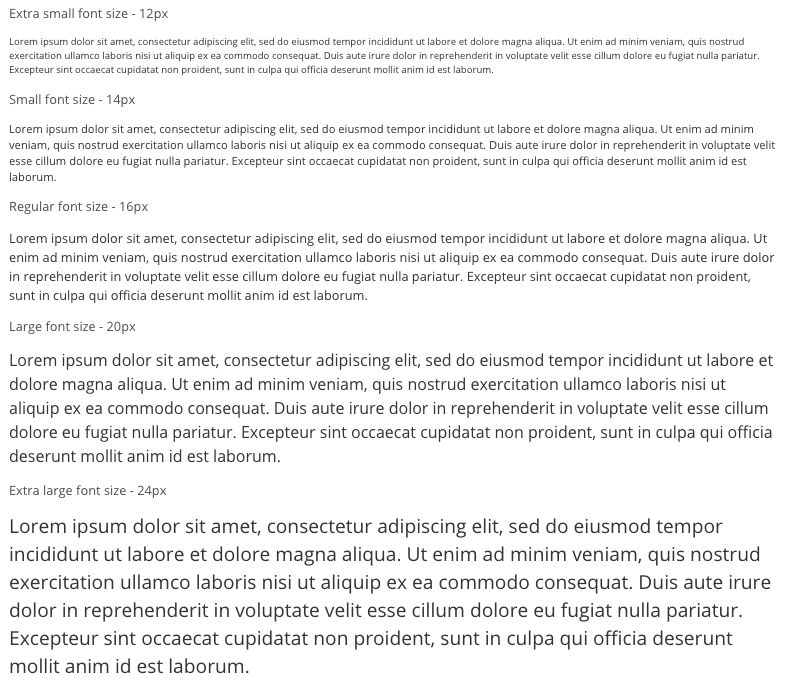
\includegraphics[scale=0.3]{images/fontsizes}
	\caption{Font Size Range}
 	\label{fig:fontSize}
\end{figure}

These classes can be called using the following methods: 

\begin{lstlisting}[language=HTML]
<p class="extra-small-p">Text</p>      
<p class="small-p">Text</p>      
<p class="large-p">Text</p>       
<p class="extra-large-p">Text</p>
\end{lstlisting}

The text can be aligned; left aligned, right aligned or justified as seen on Figure.~\ref{fig:textalign} on  page~\pageref{fig:textalign}. These classes can be called directly from the paragraph tag.

\begin{figure}[h]
\centering
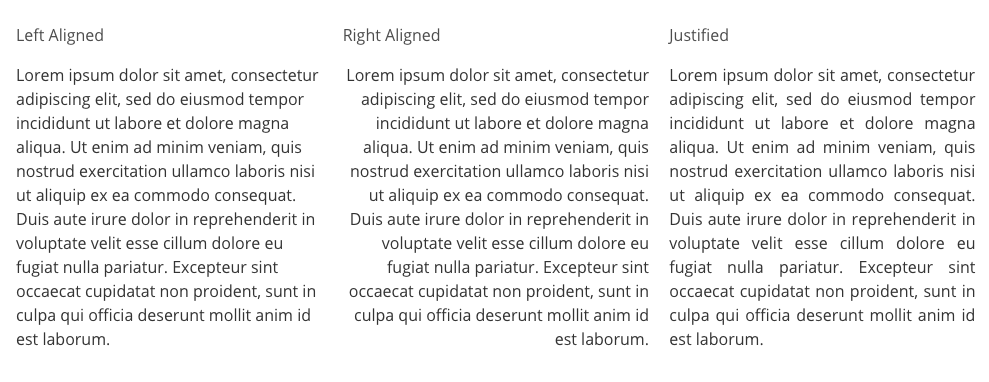
\includegraphics[scale=0.2]{images/text-align}
	\caption{Text Alignments}
    \label{fig:textalign}
\end{figure}

These classes can be called using the following methods:

 \begin{lstlisting}[language=HTML]
<p class="left-align-text"></p>
<p class="right-align-text"></p>
<p class="justified-text"></p>
\end{lstlisting}

There are four different types of font weightings as seen on Figure.~\ref{fig:fontweight} on  page~\pageref{fig:fontweight}. These font weightings can be used on paragraph, label, and heading texts.

\begin{figure}[h]
\centering
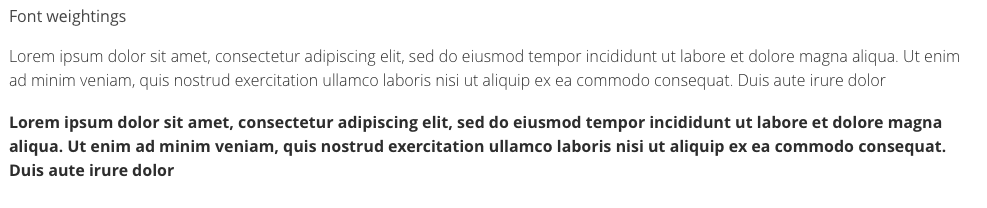
\includegraphics[scale=0.3]{images/font-weighting}
	\caption{Font Weighting}
  	\label{fig:fontweight}
\end{figure}

These weightings range from thin to bold. These classes can be called using the following methods:

\begin{lstlisting}[language=HTML]
<p class="thin-p">Text</p>
<p class="bold-p">Text</p>
\end{lstlisting}

The default font weighting for the paragraph text is 400. To change the weighting of the font, you can change the number value at the end of the variable. To save confusion, it would also be a good idea to change the variable name as seen below.

\begin{lstlisting}[language=HTML]
$font-weight-400: 400; //default
\end{lstlisting}

\begin{lstlisting}[language=HTML]
$font-weight-400: 700; //bolder
\end{lstlisting}

\newpage
\subsection*{Buttons}
\addcontentsline{toc}{subsection}{1.2 Buttons}

There are four button types in Taylor'd UI as seen in Figure.~\ref{fig:genButtons} on  page~\pageref{fig:genButtons}. These button types are styled in a similar way to how a browser would display a button. 

\begin{figure}[h]
\centering

\includegraphics[scale=0.3]{images/generic-buttonsa}
\caption{Generic Button Types}
  \label{fig:genButtons}
\end{figure}

These classes can be called using the following methods:

\begin{lstlisting}[language=HTML]
 <button class="button">Test Button</button>
<button class="pill-shaped-button">Test Button</button>
\end{lstlisting}

Additionally, a button can be styled using modifier classes. These modifiers are based on the primary colours as seen in Figure.~\ref{fig:buttonMods} on  page~\pageref{fig:buttonMods}. These colours are colours that a user would have seen in other applications used for alerts such warning, and success actions. 

\begin{figure}[h]
\centering

\includegraphics[scale=0.3]{images/button-modifiers}
\caption{Button Modifiers}
  \label{fig:buttonMods}
\centering
\end{figure}


These classes can be called using the following methods:

\begin{lstlisting}[language=HTML]
<button class="button default-button">default</button>
<button class="button primary-button">primary</button>
<button class="button success-button">success</button>
<button class="button info-button">Info</button>
<button class="button warning-button">warning</button>
<button class="button danger-button">danger</button>
<button class="button link-button">button Link</button>
\end{lstlisting}

The button modifiers can be used with the generic button classes. An example on how to call these classes: 

\begin{lstlisting}[language=HTML]
<button class="large-button info-button"></button>
<button class="pill-shaped-button warning-button"></button>
\end{lstlisting}

\newpage
\subsection*{Alerts}
\addcontentsline{toc}{subsection}{1.3 Alerts}
Alerts provide user feedback based on certain actions performed by them. An alert is built using the \latinword{.alert} class, and styled with modifier classes such as seen in Figure.~\ref{fig:alerts} on  page~\pageref{fig:alerts}. 

\begin{figure}[h]
\centering
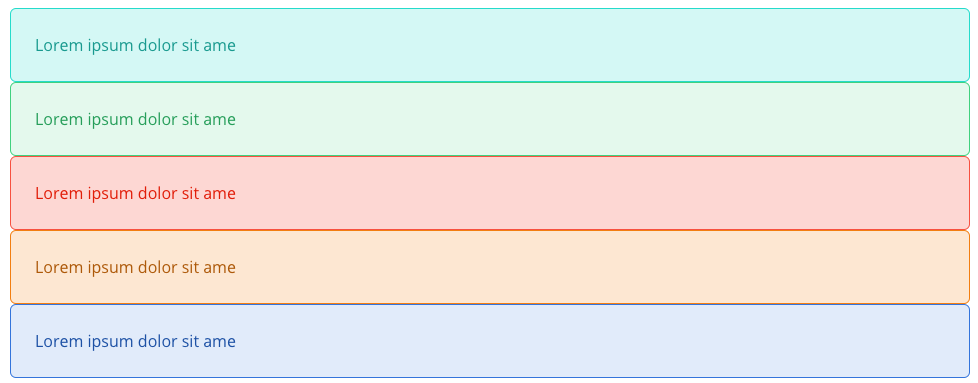
\includegraphics[scale=0.2]{images/alertd}
\caption{Alerts}
  \label{fig:alerts}
\end{figure}

An example on how these classes can be called using the following methods: 

\begin{lstlisting}[language=HTML]
<div class="alert info-alert">
<p>Lorem ipsum dolor sit ame</p>
<div class="alert success-alert">
<p>Lorem ipsum dolor sit ame</p>
so please pay attention.</p></div>
\end{lstlisting}

An alert class can be built upon by adding buttons, see Figure.~\ref{fig:AlertModifiers} on  page~\pageref{fig:AlertModifiers} as well as links.

\begin{figure}[h]
\centering
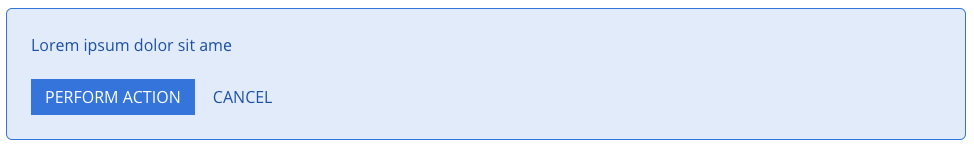
\includegraphics[scale=0.2]{images/addtoalert}
\caption{Alert Modifiers}
  \label{fig:AlertModifiers}
\end{figure}

An example on how these classes can be called using the following methods: 

\begin{lstlisting}[language=HTML]
<div class="alert alert-primary">
<p>Lorem ipsum dolor sit ame</p>
<button class="button button-primary">Do Some Action</button>
 <button class="button button-link">Cancel</button>
\end{lstlisting}

\subsection*{Tables}
\addcontentsline{toc}{subsection}{1.4 Tables}
A table allow web authors to arrange data such as text, images, links, even other tables into rows and columns of cells. The tables are created using the table tag in which the \latinword{tr} tag is used to create table rows and td tag is used to create data cells.

A default table was created for Taylor'd UI. The default table is simple, with clear emphasis on the headings of the table. 

\begin{lstlisting}[language=HTML]
<table class="table">
	<thead>
		<tr>
			<th>Lorem ipsum dolor sit ame</th>
			<th>consectetur adipiscing elit</th>
			<th>Quasi vero</th>
		</tr>
	</thead>
	<tbody>
		<tr>
			<td>inquit</td>
			<td>perpetua oratio rhetorum solum</td>
			<td>non etiam philosophorum sit</td>
		</tr>
		<tr>
			<td>magna dissensio</td>
			<td>In contemplatione et cognitione</td>
			<td>Num igitur dubium es</td>
		</tr>
		<tr>
			<td>Non est ista</td>
			<td>inquam</td>
			<td>Piso</td>
		</tr>
	</tbody>
</table>
\end{lstlisting}

There are four modifiers see Figure.~\ref{fig:tableMod} on  page~\pageref{fig:tableMod} that can be added to the table class for a different look as seen below. The other modifiers are hover-on-table,  bordered-table.

\newpage

\begin{figure}[ht]
\centering
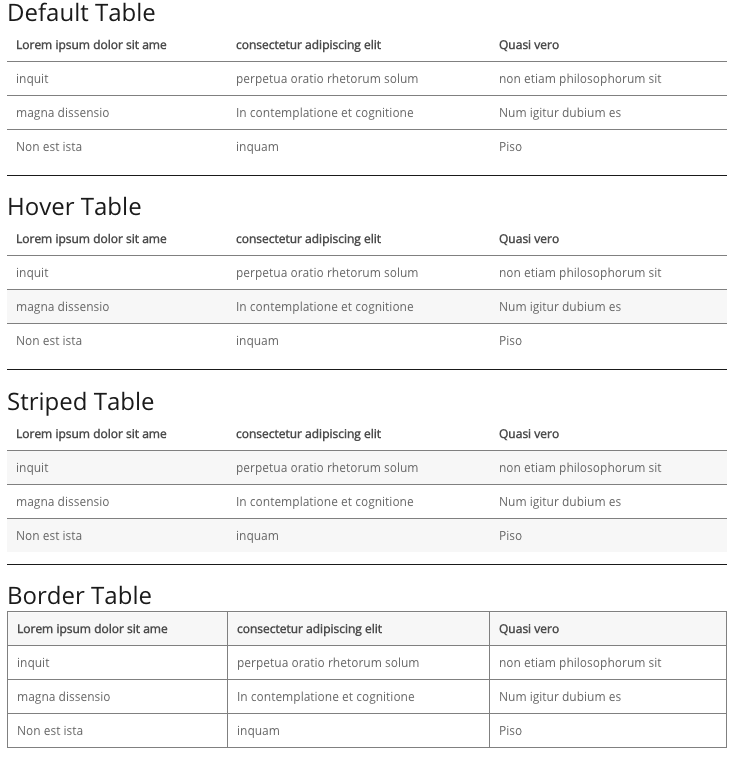
\includegraphics[scale=0.24]{images/tables}
\caption{Tables with Modifiers}
  \label{fig:tableMod}
\end{figure}

Below is an example of how to call one of the modifiers. 

\begin{lstlisting}[language=HTML]
<table class="table striped-table">
	<thead>
		<tr>
			<th>Lorem ipsum dolor sit ame</th>
			<th>consectetur adipiscing elit</th>
			<th>Quasi vero</th>
		</tr>
	</thead>
	<tbody>
		<tr>
			<td>inquit</td>
			<td>perpetua oratio rhetorum solum</td>
			<td>non etiam philosophorum sit</td>
		</tr>
		<tr>
			<td>magna dissensio</td>
			<td>In contemplatione et cognitione</td>
			<td>Num igitur dubium es</td>
		</tr>
		<tr>
			<td>Non est ista</td>
			<td>inquam</td>
			<td>Piso</td>
		</tr>
</tbody></table>
\end{lstlisting}


\newpage
Modifiers from other components such as alerts can be used on table elements, as seen on Figure.~\ref{fig:tableClass} on  page~\pageref{fig:tableClass}. 

\begin{figure}[h]
\centering
  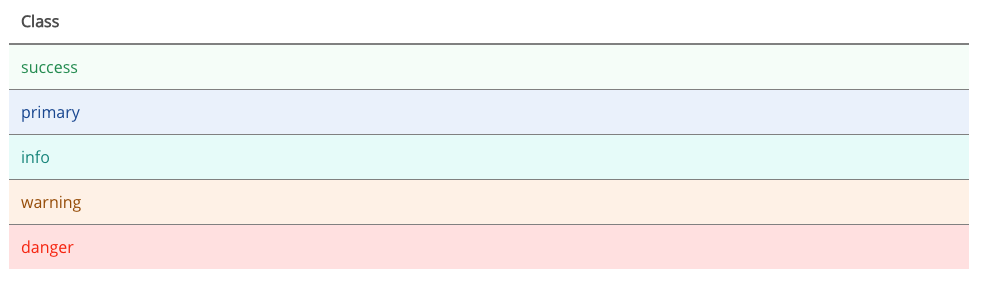
\includegraphics[scale=0.2]{images/tableClass}
\caption{Table with other Class Modifiers}
  \label{fig:tableClass}
\end{figure}

The code snippet below shows you how to call the different modifiers. 

\begin{lstlisting}[language=HTML]
<table class="table">
	<thead>
		<tr>
			<th>Modifiers</th>
		</tr>
	</thead>
	<tbody>
		<tr class="is-success">
			<td>success</td>
		</tr>
		<tr class="is-primary">
			<td>primary</td>
		</tr>
		<tr class="is-info">
			<td>info</td>
		</tr>
		<tr class="is-warning">
			<td>warning</td>
		</tr>
		<tr class="is-danger">
			<td>danger</td>
		</tr>
	</tbody>
</table>
\end{lstlisting}

\newpage
\subsection*{Panels}
\addcontentsline{toc}{subsection}{1.5 Panels}
A panel in Taylor'd UI is a bordered box with some padding around its content. The basic panel is just that, see Figure.~\ref{fig:panel} on  page~\pageref{fig:panel}. Other attributes such as heading tags can be added to a panel as seen below: 

\begin{figure}[h]
\centering
  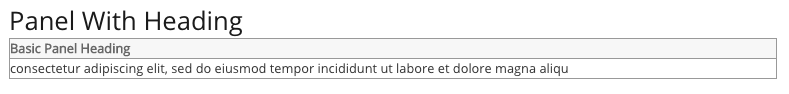
\includegraphics[scale=0.28]{images/panel}
  \caption{Default Panel}
  \label{fig:panel}
\end{figure}


\begin{lstlisting}[language=HTML]
<div class="panel default-panel">
	<div class="panel-title">Lorem Ipsumn
	</div>
	<div class="panel-body"> consectetur adipiscing elit, 
	sed do eiusmod tempor incididunt ut labore et dolore magna aliqu
	</div>
</div>
\end{lstlisting}

Modifiers from other components such as alerts see Figure.~\ref{fig:panelmod} on  page~\pageref{fig:panelmod} can be added to a panel. The code snippet below shows you one example: 

\begin{figure}[h]
\centering
  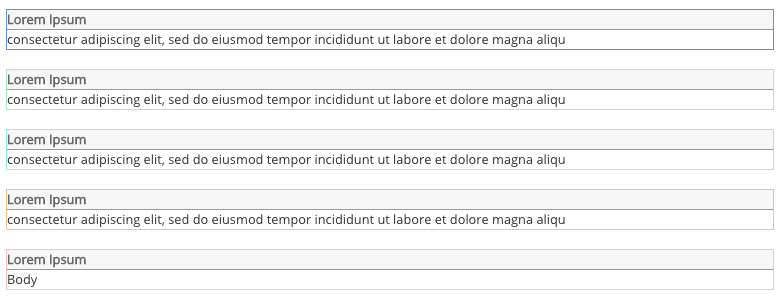
\includegraphics[scale=0.27]{images/panelmod}
\caption{Panel with Modifiers}
  \label{fig:panelmod}
\end{figure}

\begin{lstlisting}[language=HTML]
<div class="panel panel-info">
	<div class="panel-title">orem Ipsum</div>
	<div class="panel-body"> consectetur adipiscing elit, 
	sed do eiusmod tempor incididunt ut labore et dolore magna aliqu
	</div>
</div>
\end{lstlisting}


\subsection*{Labels}
\addcontentsline{toc}{subsection}{1.6 Labels}

Labels are built with button-label class, the default label does not need the button class, as seen below: 

\begin{lstlisting}[language=HTML]
<span class="button-label">Default Label</span>
\end{lstlisting}

Modifiers can be added to the label see Figure.~\ref{fig:label} on  page~\pageref{fig:label} for more impact.

\begin{figure}[h]
\centering
  
\includegraphics[scale=0.5]{images/labels}
\caption{Labels}
  \label{fig:label}
\end{figure}


An example on how these classes can be called using the following methods: 

\begin{lstlisting}[language=HTML]
<span class="button-label">Default Label</span>
<span class="button-label primary">Default Primary</span>
<span class="button-label success">Success Label</span>
<span class="button-label info">Info Label</span>
<span class="button-label warning">Warning Label</span>
<span class="button-label danger">Danger Label</span>
\end{lstlisting}

\newpage
\subsection*{Jumbotron}
\addcontentsline{toc}{subsection}{1.7 Jumbotron}
Jumbotrons can be treated as large panels, the default panel has the text entered in the centre with lots of padding all round, as seen in Figure.~\ref{fig:jumbo} on  page~\pageref{fig:jumbo}. 


\begin{figure}[h]
\centering
  
\includegraphics[scale=0.4]{images/jumbrotron}
  \caption{Jumbotron}
  \label{fig:jumbo}
\end{figure}

Below is the code needed to create a jumbotron: 

\begin{lstlisting}[language=HTML]
<div class="jumbotron"><h1>Lorem Ipsum</h1></div>
\end{lstlisting}

As jumbotrons share similar attributes to panels, the same modifiers that apply to panels can also be applied here as seen in Figure.~\ref{fig:jumbowithmod} on  page~\pageref{fig:jumbowithmod}. 

 \begin{figure}[h]
\centering
  
\includegraphics[scale=0.4]{images/jumbowithmod}
  \caption{Jumbotron with Modifier}
  \label{fig:jumbo}
\end{figure}

\begin{lstlisting}[language=HTML]
<div class="jumbotron alert-primary"><h1>Lorem Ipsum</h1></div>
\end{lstlisting}

\subsection*{Button Groups / Pagination}
\addcontentsline{toc}{subsection}{1.8 Button Groups / Pagination}
Button groups are a collection of buttons on the same line. Button groups work in the same way that buttons work as seen in Figure.~\ref{fig:defualtgroup} on  page~\pageref{fig:defualtgroup}. To group a collection of buttons, add the class button-group around the collection . 


\begin{figure}[h]
\centering
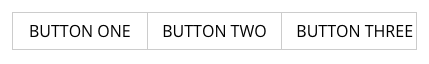
\includegraphics[scale=0.3]{images/button-group=defualt}
\caption{Default Button Group}
  \label{fig:defualtgroup}
\end{figure}

Below is an example of the default button group: 

\begin{lstlisting}[language=HTML]
<div class="button-group"><button class="button button-default">
Button One</button>
<button class="button default-button">Button Two</button>
<button class="button default-button">Button Three</button>
</div>
\end{lstlisting}

As with buttons, the same modifiers, see Figure.~\ref{fig:groupSize} on  page~\pageref{fig:groupSize} can be added to either increase the button-group size. 

\begin{figure}[h]
\centering
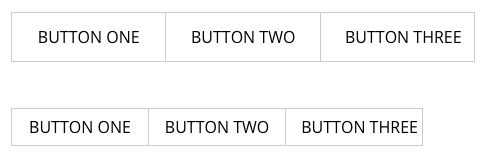
\includegraphics[scale=0.3]{images/button-group-size}
\caption{Button Group Sizes}
  \label{fig:groupSize}
\end{figure}


The code snippet below shows you the large button group:

\begin{lstlisting}[language=HTML]
<div class="button-group large-button-group">
	<button class="button default-button">Button One</button>
	<button class="button default-button">Button Two</button>
	<button class="button default-button">Button Three</button>
</div>
\end{lstlisting}

Or adding colour to the group see Figure.~\ref{fig:modButtonGroup} on  page~\pageref{fig:modButtonGroup}. 

\begin{figure}[h]
\centering

\includegraphics[scale=0.3]{images/buttongroups}
\caption{Button Group With Modifiers}
  \label{fig:modButtonGroup}
\end{figure}

Below is one example of modifiers:  

\begin{lstlisting}[language=HTML]
<div class="button-group">
<button class="button primary-button">Button One</button>
<button class="button primary-button">Button Two</button>
<button class="button primary-button">Button Three</button>
</div>
\end{lstlisting}

\subsection*{Forms}
\addcontentsline{toc}{subsection}{1.9 Forms}
There are multiple elements that make up a form. Taylor'd UI caters for all these elements. The overall styling for the form comes from the form-styling class as seen below:

\begin{lstlisting}[language=HTML]
<div class="form-styling"></div>
\end{lstlisting}

The following inputs make the overall form see Figure.~\ref{fig:form} on  page~\pageref{fig:form}. Passwords are not entered in as plain text as the type has been set to passwords, allowing for asterisks to appear instead. All form elements have placeholder text contained that when a user starts typing, the placeholder text disappears.

\begin{figure}[h]
\centering
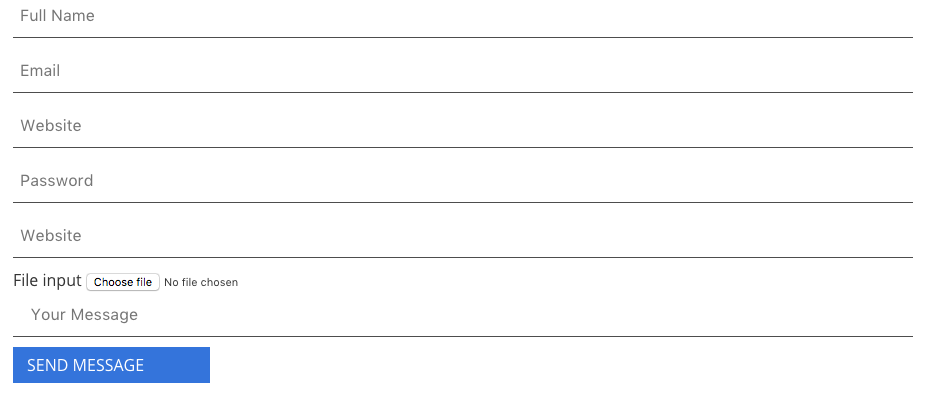
\includegraphics[scale=0.3]{images/form}
\caption{Form Elements}
  \label{fig:form}
\end{figure}


\begin{lstlisting}[language=HTML]
<input type="text" name="field1" placeholder="Full Name" />
<input type="email" name="field2" placeholder="Email" />
<input type="url" name="field3" placeholder="Website" />
<input type="password" id="password_id" placeholder="Password">
<input type="number" name="field4" placeholder="Website" />
<label for="someFile">File input</label>
<input type="file" id="fileUpload">
<textarea placeholder=" Your Message" 
onkeyup="adjust_textarea(this)"></textarea>
<input class="button button-primary" value="Send Message" />
\end{lstlisting}

Other features such as radio and check boxes see figure Figure.~\ref{fig:radio} on  page~\pageref{fig:radio} have specific id's so that only one option can be checked at any given time. 

\begin{figure}[h]
\centering
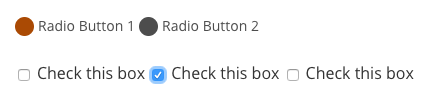
\includegraphics[scale=0.4]{images/radio}
\caption{Radio Buttons and Checkboxes}
  \label{fig:radio}
\end{figure}

Below is the two types: 

\begin{lstlisting}[language=HTML]
<input type="radio" id="radio01" name="radio" />
<label for="radio01"><span></span>Radio Button 1</label>
<input type="radio" id="radio02" name="radio" />
<label for="radio02"><span></span>Radio Button 2</label>
<label><input type="checkbox"> Check this box</label>
<label><input type="checkbox"> Check this box</label>
<label><input type="checkbox"> Check this box</label>
\end{lstlisting}

\newpage
\subsection*{Navigation}
\addcontentsline{toc}{subsection}{1.10 Navigation}
The \latinword{nav} tag defines a set of navigation links. The \latinword{nav} tag is only intended for a block of high level links, this helps screen readers determine whether or not to render the content.

The navigation bar in Taylor'd UI is kept simple in keeping with the ethos of non-opinionated design as seen in Figure.~\ref{fig:nav} on  page~\pageref{fig:nav}. The nav bar has been designed to always stay on top when a user is browsing a site on Desktop type devices. On mobile devices, the navigation bar disappears as the user scrolls a website. 

\begin{figure}[h]
\centering
  
\includegraphics[scale=0.2]{images/nav}
  \caption{Navigation Bar}
  \label{fig:nav}
\end{figure} 

In keeping with best practices, the nav should be called within a header tag as seen below:

\begin{lstlisting}[language=HTML]
  <header>
    <a href="#" id="logo"></a>
    <nav>
      <a href="#" id="menu-icon"></a>
      <ul>
        <li><a href="#" class="current">Home</a></li>
        <li><a href="#">About</a></li>
        <li><a href="#">Work</a></li>
        <li><a href="#">Blog</a></li>
        <li><a href="#">Contact</a></li>
      </ul>
    </nav>
  </header>
\end{lstlisting}

\newpage
\subsection*{960 grid, 12 column system}
\addcontentsline{toc}{subsection}{1.11 960 grid, 12 column system}
Taylor'd UI is based on a 960 grid system. The grid system of 12 grids. 12 columns is used as each column can be evenly divided by 960. This allows the end user to build a seamless experience from desktops to mobile devices.

The columns are also used to layout the content of a web page as seen in Figure.~\ref{fig:columnlayout} on  page~\pageref{fig:columnlayout}. When using columns, it is important to remember that the columns in the section you are using them in, always match up to 12.

\begin{figure}[h]
\centering
  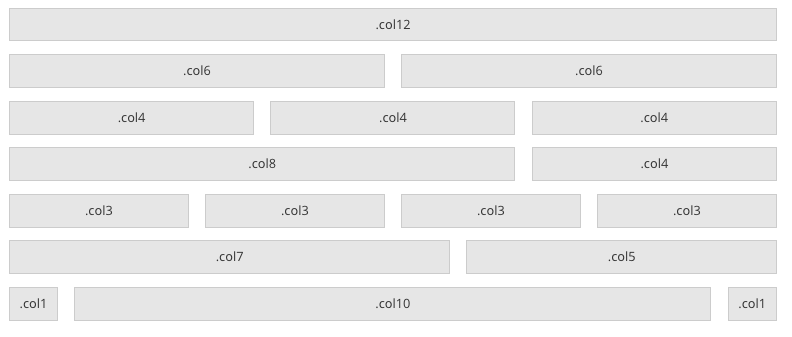
\includegraphics[scale=0.4]{images/columnlayout}
  \caption{12 Column Layout}
  \label{fig:columnlayout}
\end{figure} 

The class row-fluid is used to make the layout more fluid across devices. Media queries are also used to ensure that Taylor'd UI components collapse when they need to as seen in Figure.~\ref{fig:collapsed} on  page~\pageref{fig:collapsed}. 


